\begin{figure}
    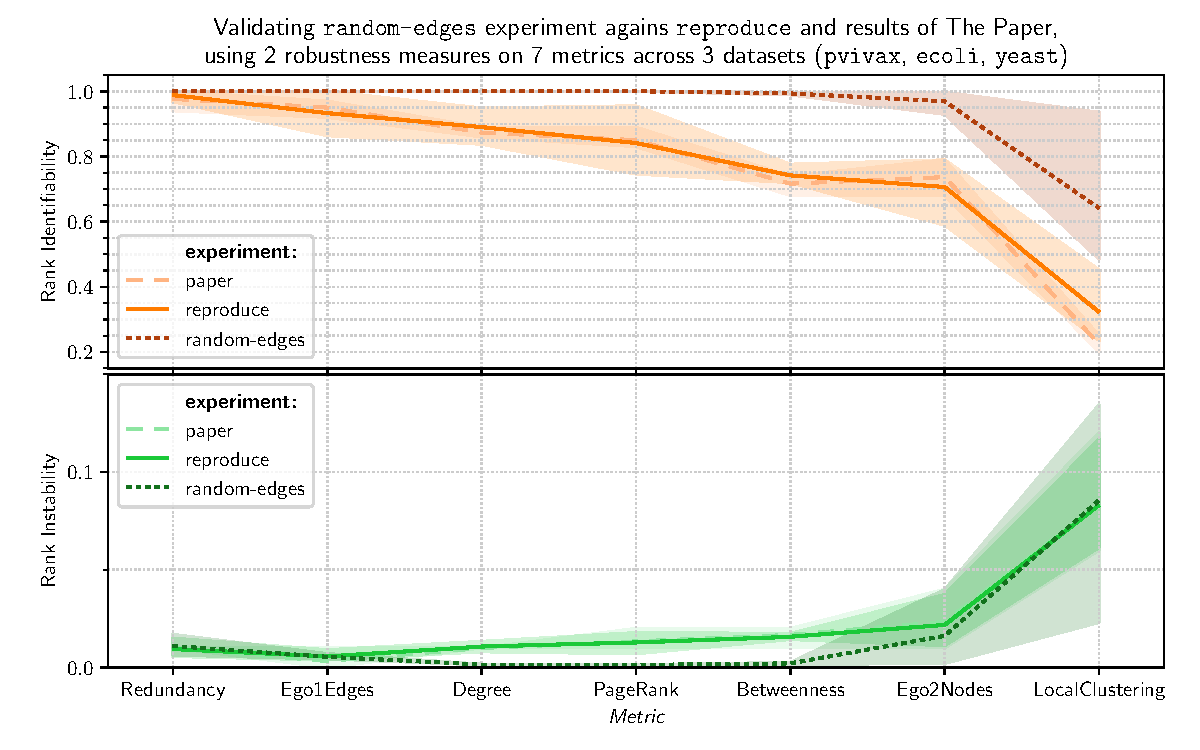
\includegraphics[width=\linewidth]{plot_random_edges.pdf}
    \vspace*{-0.6cm}
    \caption{Validation of the \texttt{random-edges} experiment against \texttt{reproduce} and results of The Paper, using RankIdentifiability and RankInstability (displayed separately) on 7 metrics across 3 datasets.
    Thin lines inside each color band band show robustness of individual datasets, and the thick line shows the average robustness across the 3 datasets.
    Each line style (solid, long dashes, short dashes) corresponds to results obtained from different experiment or source.}
    \label{fig:plot_random_edges}
    \footnotesize
    \begin{flushleft}
        High values of RankIdentifiability mean high \textsl{robustness}, whereas high values of RankInstability mean low \textsl{robustness}.
        Metrics are sorted from left to right by their decreasing combined robustness.
    \end{flushleft}
\end{figure}
